\documentclass{beamer}
\usepackage{beamerthemesplit} % new

\usepackage[utf8]{inputenc}
\documentclass{beamer}
\usepackage{beamerthemesplit} % new

\usepackage[utf8]{inputenc}
\usepackage[utf8]{inputenc}
\usepackage{tikz}
\usepackage[export]{adjustbox}
\newcommand{\roundpic}[4][]{
  \tikz\node [circle, minimum width = #2,
    path picture = {
      \node [#1] at (path picture bounding box.center) {
        \includegraphics[width=#3]{#4}};
    }] {};}

\usepackage{graphicx,wrapfig,lipsum}
\usepackage{multicol}

\usepackage{tcolorbox}

\begin{document}
\title{MY NEIGH}
\author{BDBI\_2019\_GR\_04}
\date{\today}

\frame{\titlepage}

\frame{\frametitle{Table of contents}\tableofcontents}



\frame{\frametitle{Team}
  \begin{itemize}
    \item MARTA IBÁÑEZ 
    \item JUDIT CAMPS   
    \item AINA MONTALBAN 
  \end{itemize}
  \vspace{1cm}
  \hspace{2cm}
 \roundpic[xshift=-0.03cm,yshift=-0.03cm]{2cm}{2cm}{images/marta.png}
   \hspace{0.5cm}
 \roundpic[xshift=-0.03cm,yshift=-0.03cm]{2cm}{2cm}{images/judit.JPG}
    \hspace{0.5cm}
  \roundpic[xshift=-0.03cm,yshift=-0.03cm]{2cm}{2cm}{images/aina.JPG}
}


\section{Trello}
\subsection{Trello Tasks}
\frame{\frametitle{Plan}
\begin{center}
    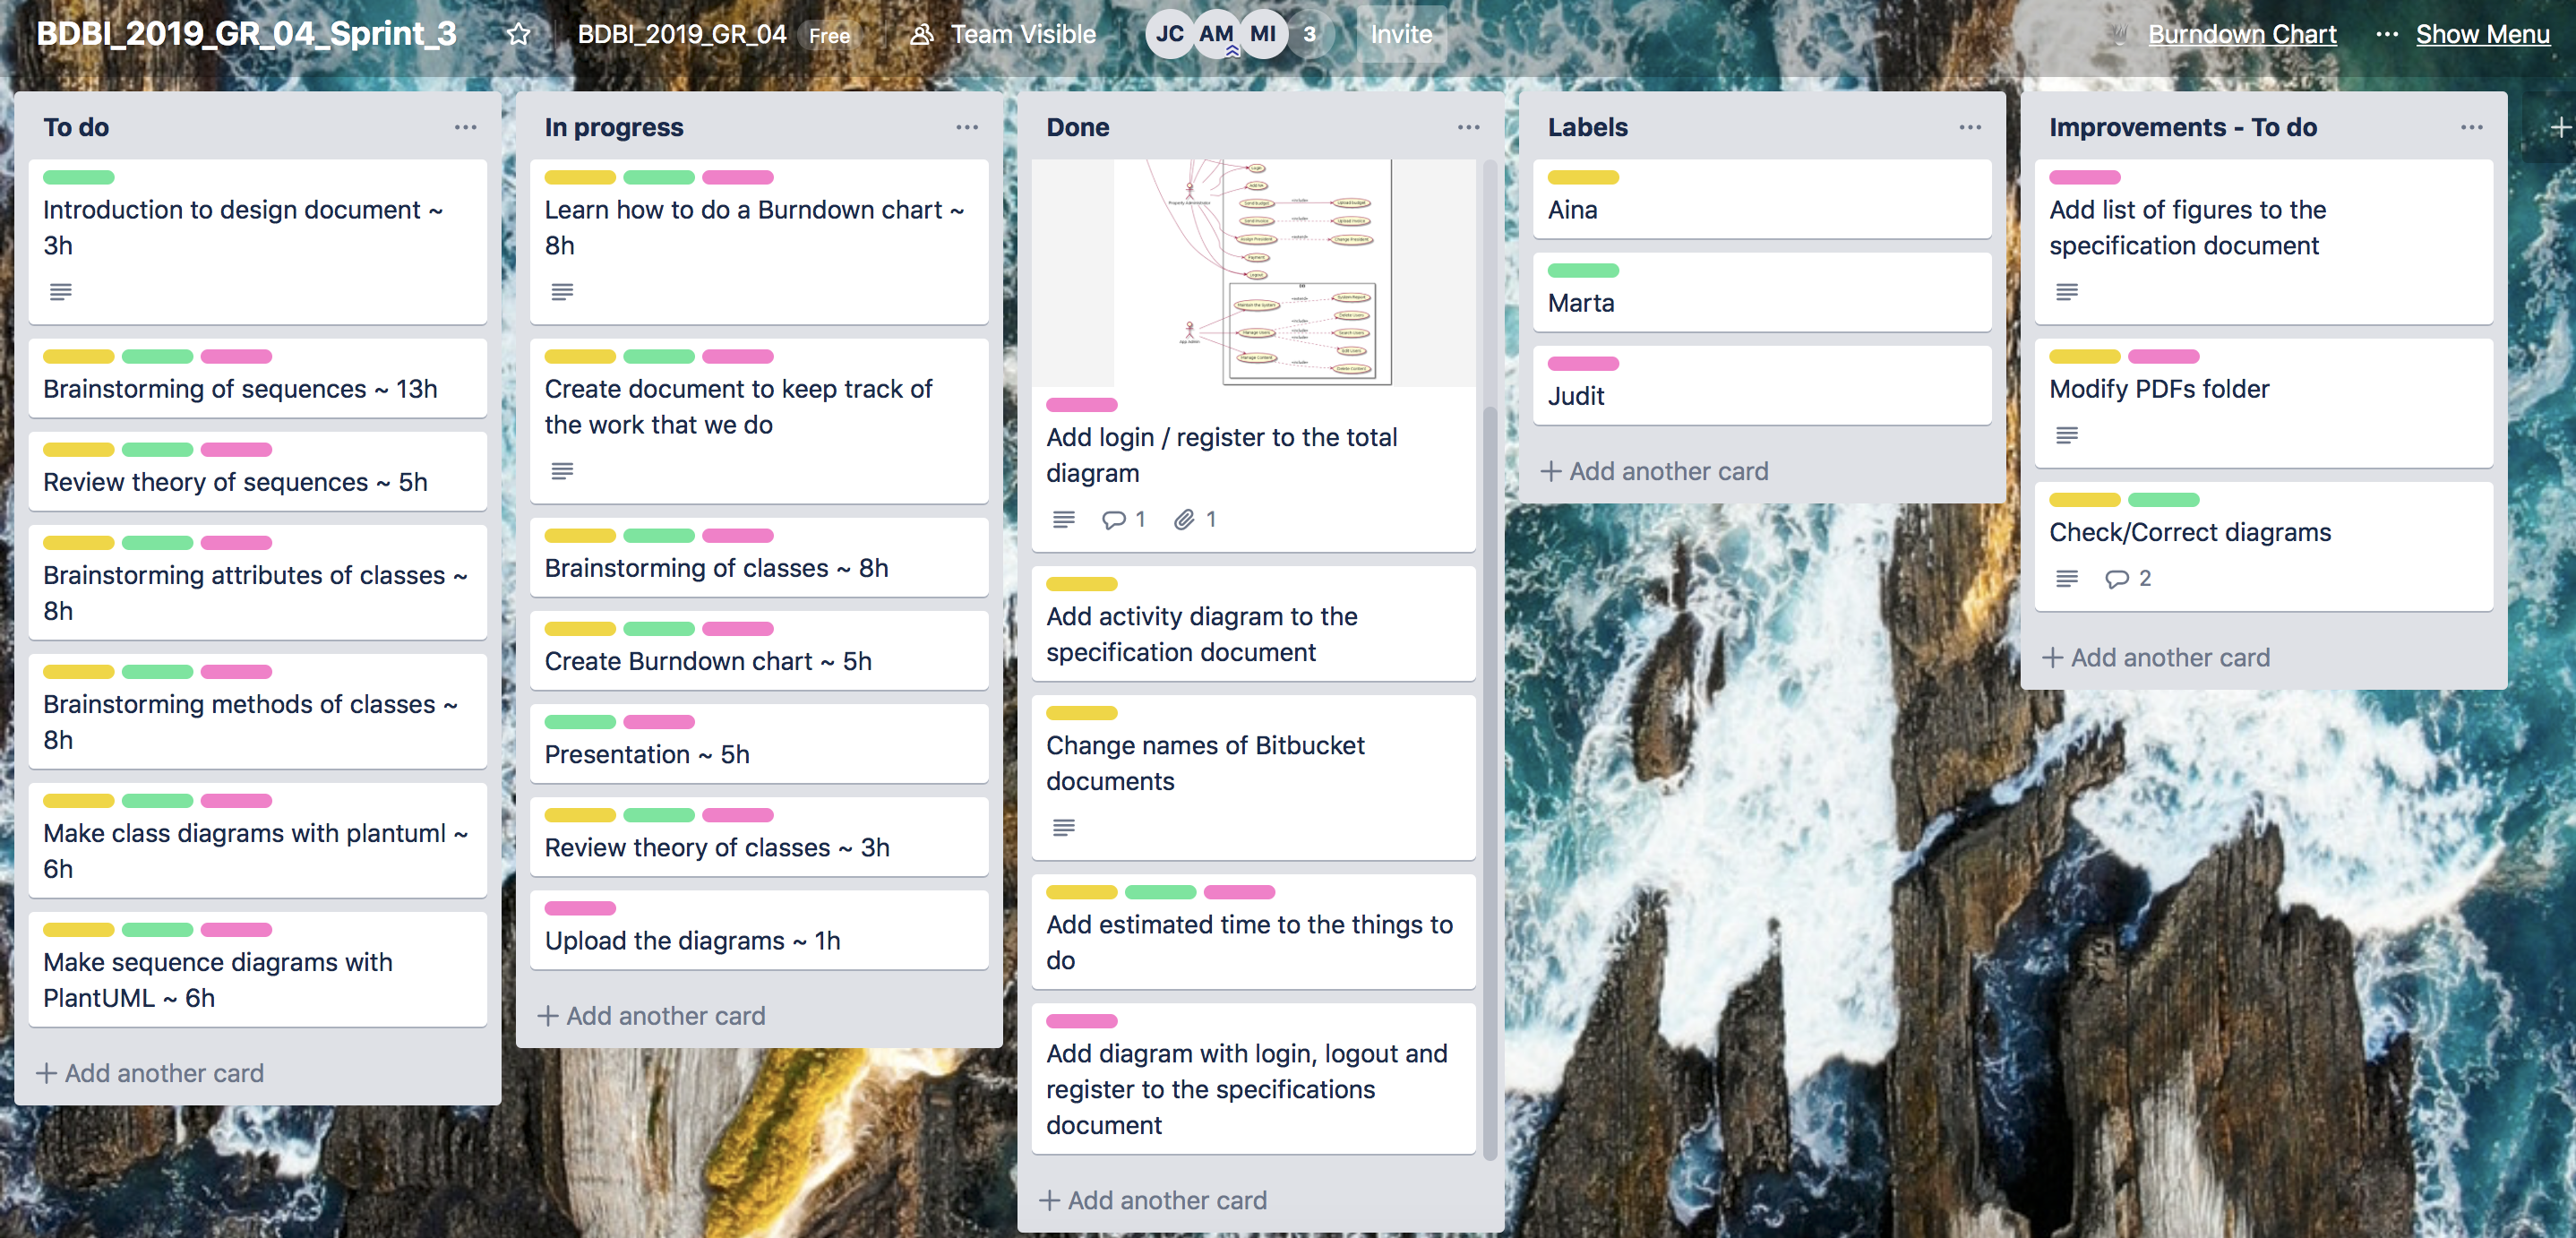
\includegraphics[scale=0.22]{Presentation/images/trello_s3.png}
\end{center}
}

\frame{\frametitle{Done}
\begin{itemize}
    \item Brainstorming of classes, attributes and methods
    \item Brainstormig of sequence diagrams
    \item Making class diagram with Plantuml
    \item Making sequence diagrams with Plantuml
    \item Check diagram errors
    \item Make presentation
\end{itemize}
}

\section{Bitbucket}
\frame{\frametitle{Bitbucket}
\begin{center}
    
\includegraphics[scale=0.2]{Presentation/images/bitbucket.png}
\end{center}
}

\section{Burndown Chart}
\frame{\frametitle{Progress}
\begin{center}
    \includegraphics[scale=0.25]{Presentation/images/burdownchart.png}
\end{center}
}

\frame{\frametitle{Class Diagram}
\begin{center}
    \includegraphics[scale=0.12]{Presentation/images/class_diagram_sprint3_1.png}
\end{center}

}
\section{Sequence diagrams}
\subsection{Adding an event to the calendar}
\frame{\frametitle{Sequence Diagram: Add event}
\begin{center}
    \includegraphics[scale=0.22]{Presentation/images/sequence_diagram_1_2.png}
\end{center}
}

\section{Conclusions}
\frame{\frametitle{Conclusions}
}

\end{document}
